\chapter{Supplementary Material}
\label{ap:supp}
\markboth{Supplementary Material}{}
\graphicspath{{image_directory/appendix/}}

\section{HLLC Riemann Solver}
\label{ap:HLLCriemann}

	In 1992 Toro \cite{Toro92} introduced a development of the HLL Riemann solver, assuming the two original waves present in HLL and inbetween adding in a contact wave\footnote{The C in HLLC stands for contact wave.}.The HLLC fluxes are also given depending on the choice of left and right wave speeds as well as an middle speed given as $S_*$. The HLLC flux is given by four regions separated by three waves,
	\begin{equation}
		\mathbf{F}=
		\begin{cases}
			\mathbf{F}_L, & if \quad 0\leq S_L, \\
			\mathbf{F}_{*L}=\mathbf{F}_L+S_L\left(\mathbf{U}_{*L}-\mathbf{U}_L\right), & if \quad S_L\leq0\leq S_*, \\
			\mathbf{F}_{*R}=\mathbf{F}_R+S_R\left(\mathbf{U}_{*R}-\mathbf{U}_R\right), & if \quad S_*\leq0\leq S_R, \\
			\mathbf{F}_R, & if \quad S_R\leq0.
		\end{cases}
		\nonumber
	\end{equation}
	The middle conserved vector $\mathbf{U}_{*K}$, for $K=L,R$, is expressed in 1D as
	\begin{equation}
		\mathbf{U}_{*K}^{1D}=\rho_K\left(\frac{S_K-u_K}{S_K-S_*}\right)
		\left[
		\begin{matrix}
			1\\
			S_*\\
			\frac{E_K}{\rho_K}+\left(S_*-u_K\right)\left(S_*+\frac{p_K}{\rho_K\left(S_K-u_K\right)}\right)
		\end{matrix}
		\right],
		\nonumber
	\end{equation}
	and in 2D as
	\begin{equation}
		\mathbf{U}_{*K}^{2D}=\rho_K\left(\frac{S_K-u_K}{S_K-S_*}\right)
		\left[
		\begin{matrix}
			1\\
			S_*\\
			v_K \\
			\frac{E_K}{\rho_K}+\left(S_*-u_K\right)\left(S_*+\frac{p_K}{\rho_K\left(S_K-u_K\right)}\right)
		\end{matrix}
		\right].
		\nonumber
	\end{equation}
	The middle wave speed $S_*$ depends on the dimension of the problem, for 1D
	\begin{equation}
		S_*^{1D}=\frac{p_R-p_L+\rho_Lu_L\left(S_L-u_L\right)-\rho_Ru_R\left(S_R-u_R\right)}{\rho_L\left(S_L-u_L\right)-\rho_R\left(S_R-u_R\right)}, \nonumber
	\end{equation}
	however in 2D, the approximate Riemann solver has the conditions \cite{Toro09},
	\begin{equation}
		u_{*L}=u_{*R}=u_*, \quad and \quad S_*=u_*, \nonumber
	\end{equation}
	so the middle wave speed in 2D is
	\begin{equation}
		S_*^{2D}=u_*. \nonumber
	\end{equation}
	All flow variables in the left or right states, including left and right fluxes, can be calculated from the variables given in the conserved vector $\mathbf{U}$.

\section{Nagel-Schreckenberg Model}
\label{ap:nagsch}

	See Section \ref{sec:nagschreck}, and code in Appendix \ref{code:NaSc}.

	\begin{figure}[H]
  		\centering
  		\subfloat[Physical location]{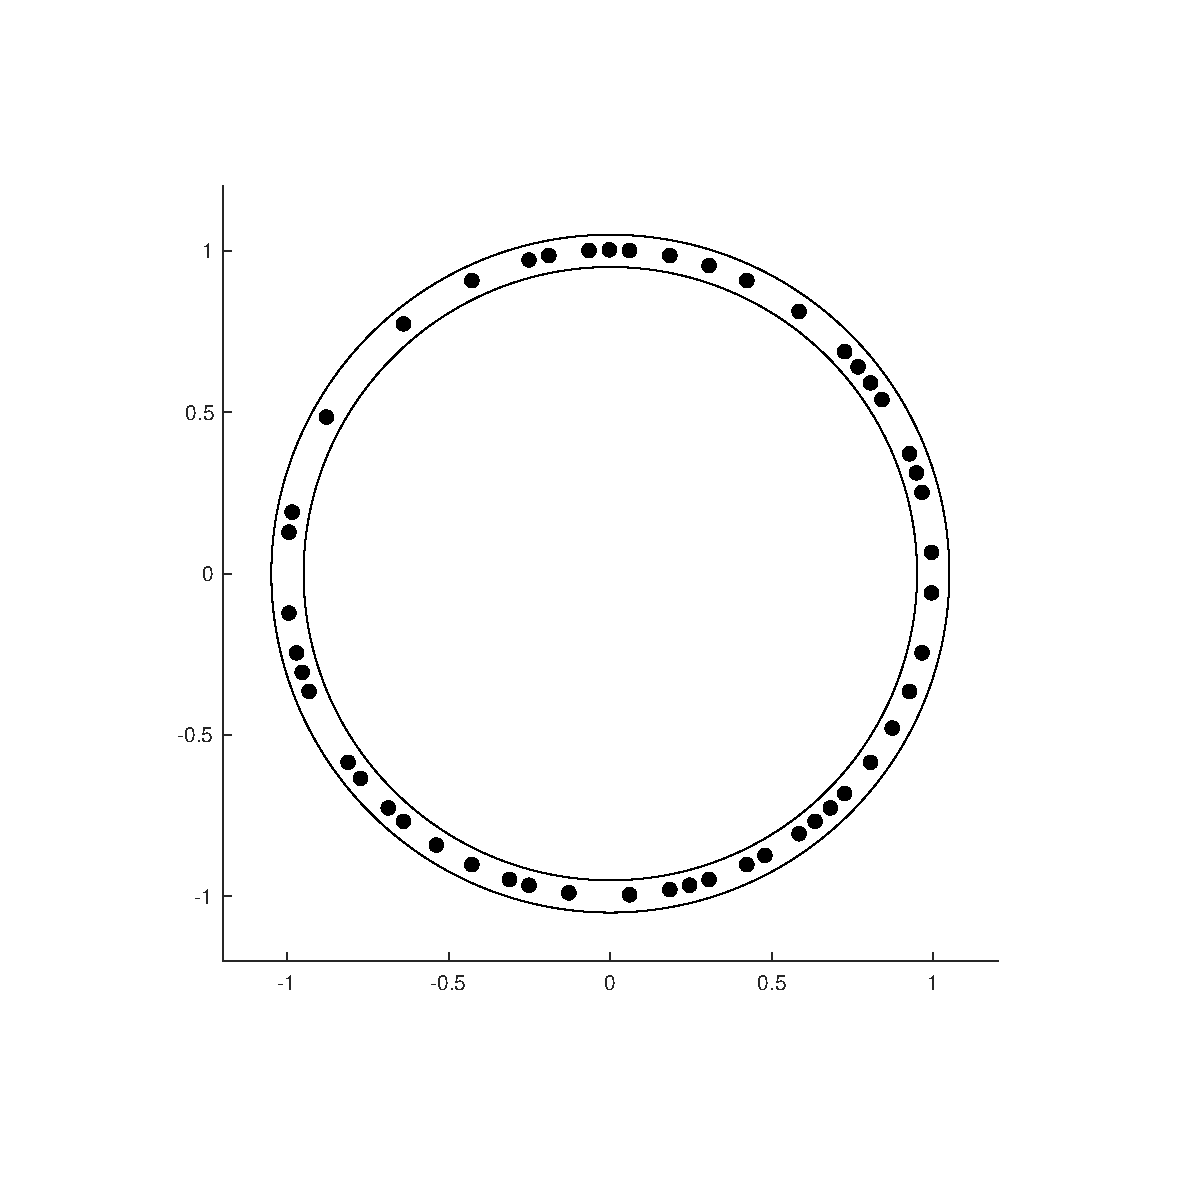
\includegraphics[trim=50 70 60 70,clip,width=0.49\textwidth]{NS_physical.pdf}\label{fig:supp:NaSc:phys}}
  		\hfill
  		\subfloat[Pathline clustering waves]{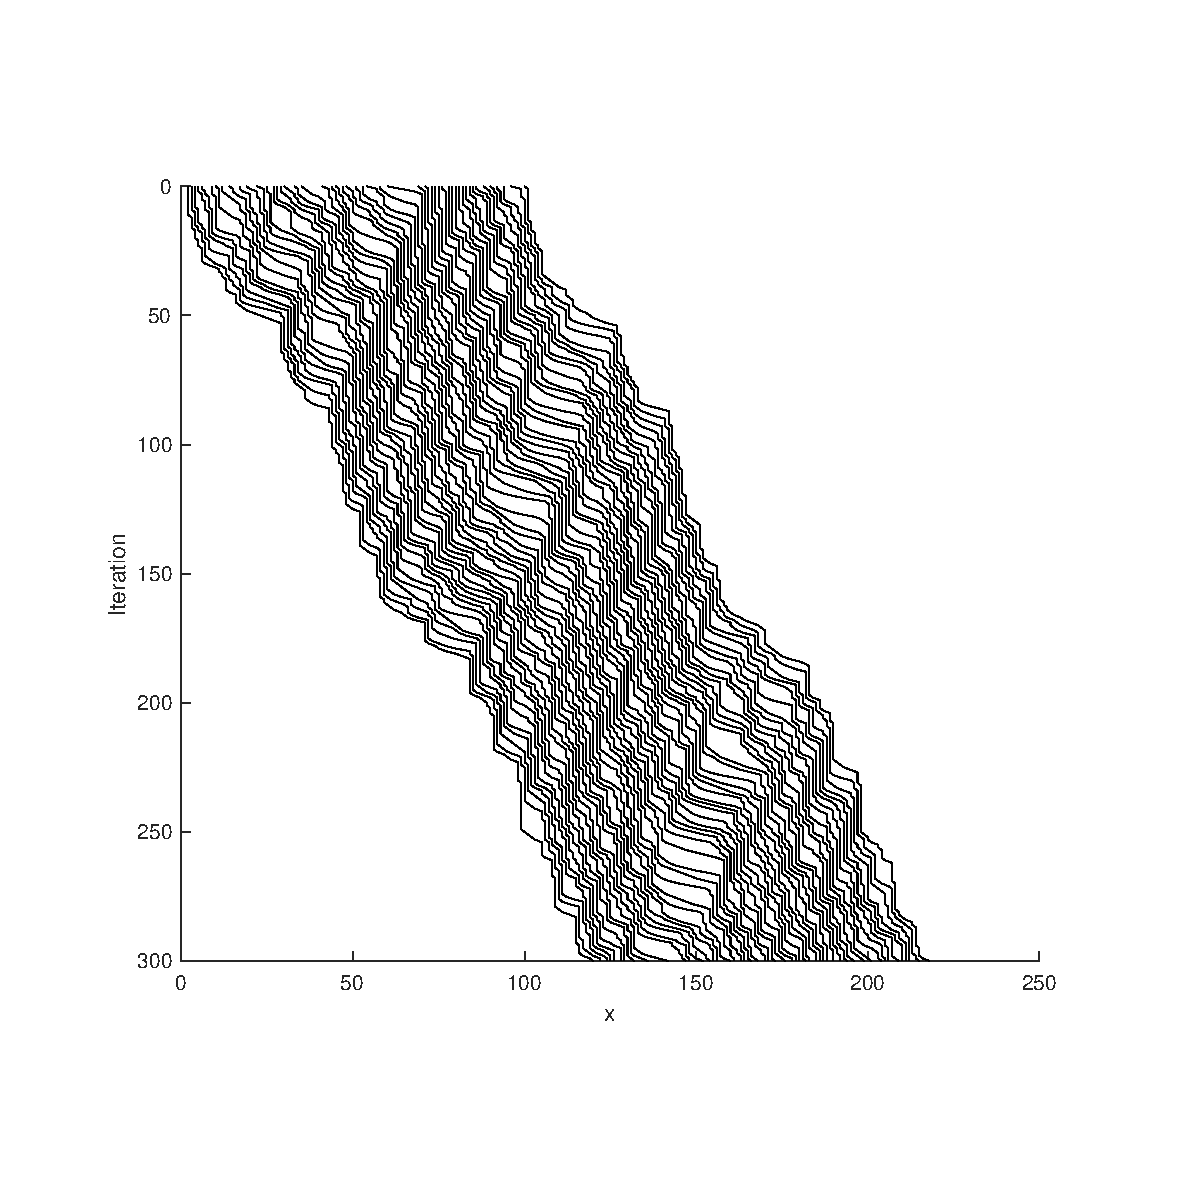
\includegraphics[trim=50 70 60 70,clip,width=0.49\textwidth]{NS_waves.pdf}\label{fig:supp:NaSc:wav}}
  		\caption[Nagel-Schreckenberg simulation]{Results from 300 iterations of the Nagel-Schreckenberg \cite{Nagel92} model. Figures show physical position on a circular road (a), and displacement $x$ from the road origin traced by iteration to show phantom traffic jams. \label{fig:aupp:NaSc}}
	\end{figure}

\newpage
\section{Genealogical Traffic Flow Model Tree}

	\begin{figure}[H]
    		\centering
        		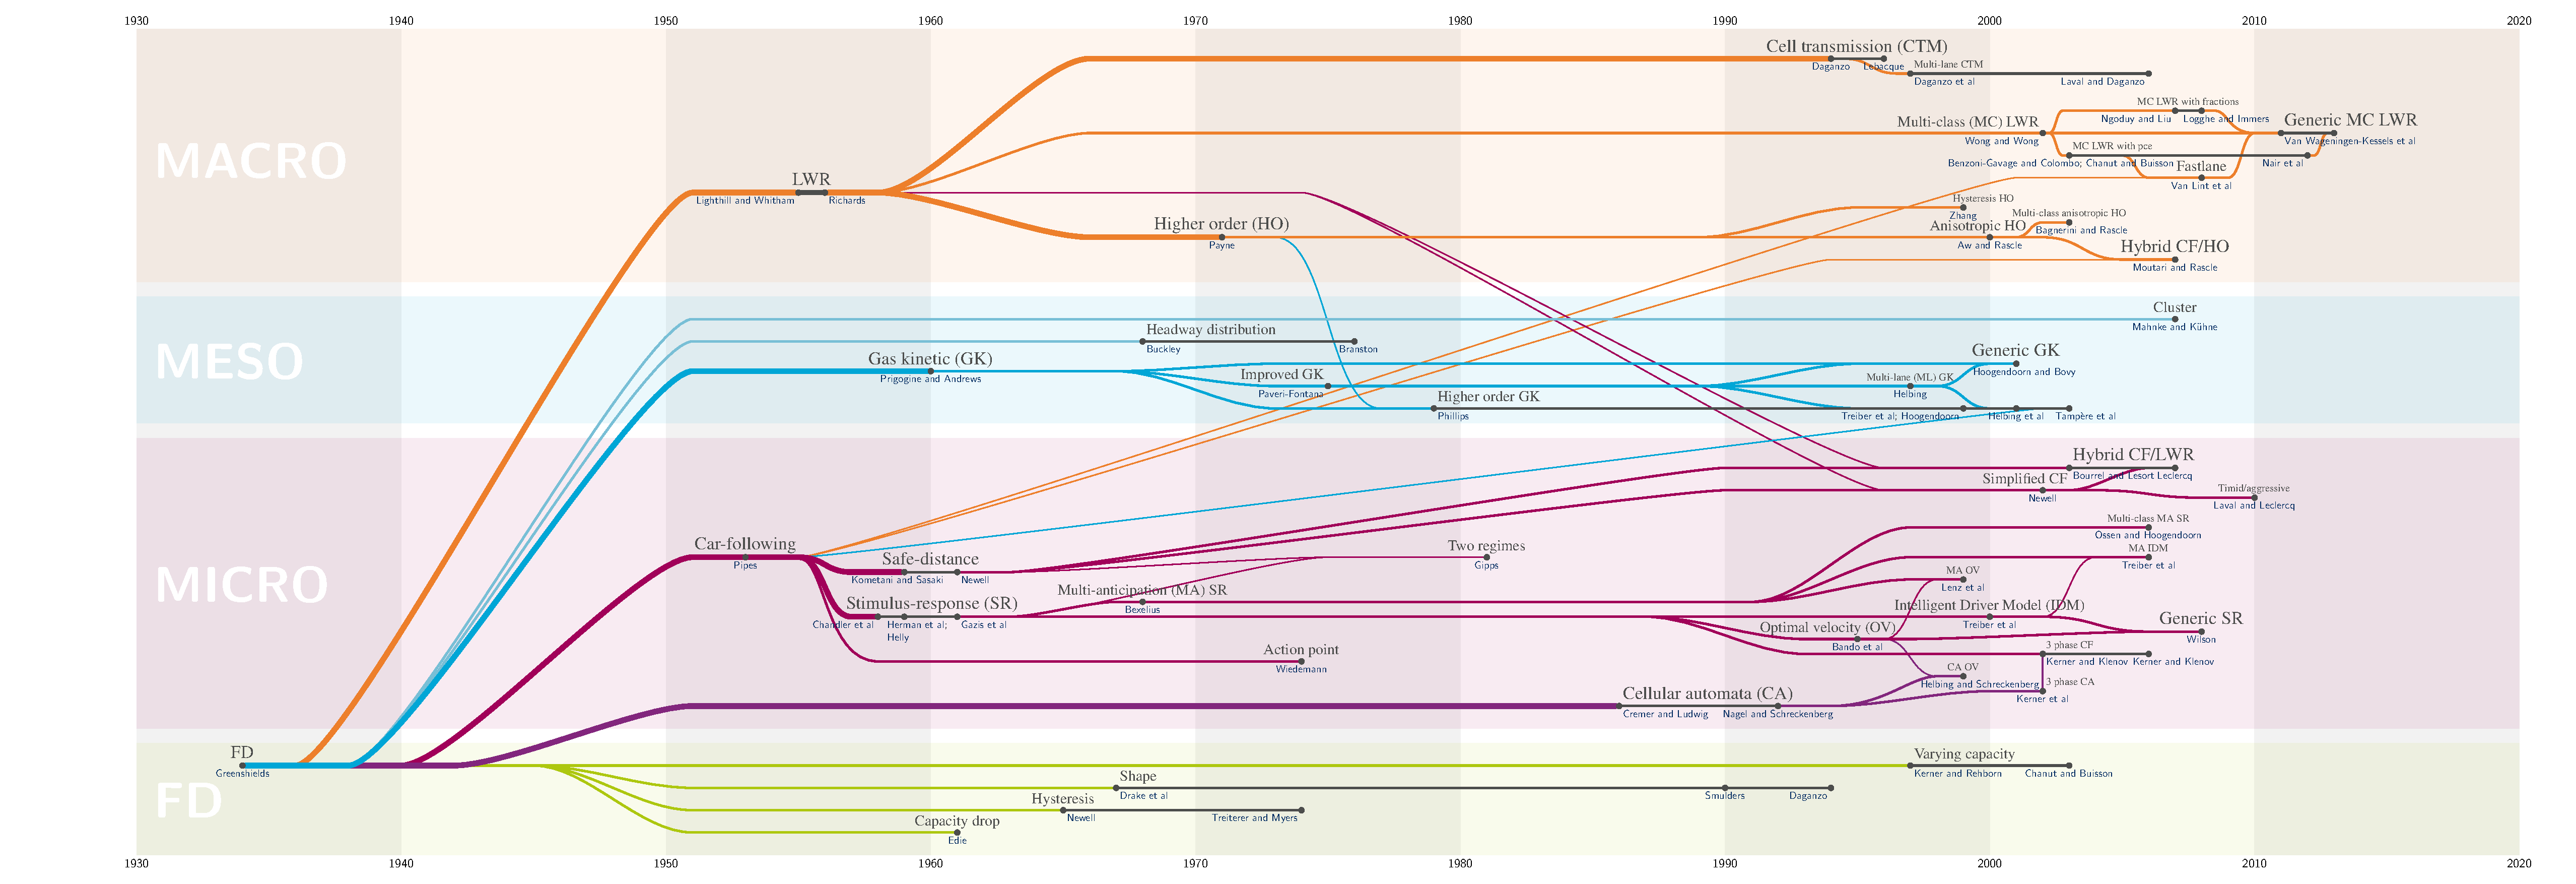
\includegraphics[angle=90,origin=c,trim=0 0 0 0,clip,height=0.9\textwidth]{TFM_timeline.pdf}
		\caption[Genealogical model tree]{Part of the online access \cite{Kessels15} (doi: \href{https://doi.org/10.1007/s13676-014-0045-5}{\texttt{10.1007/s13676-014-0045-5}}) includes a full size version complete with references.}
		\label{fig:supp:tree}
	\end{figure}
	
\newpage
\section{Simulation Information Output}
\lstset{inputpath=textfiles/}
\label{txt:info:output} 

\subsection{Written Text File}
\label{txt:info:file} 
	\lstset{style=txt}
	\lstinputlisting[firstline=0,lastline=49]{simulation_info.txt}

\subsection{Console}
\label{txt:info:console} 
	\lstset{style=txt}
	\lstinputlisting[firstline=0,lastline=8]{console.txt}







